\documentclass[11pt,a4paper]{article}
\usepackage[english]{babel}
\usepackage[square,numbers]{natbib}
\bibliographystyle{abbrvnat}
\usepackage[margin=1in]{geometry}

\usepackage{subcaption}
\usepackage{graphicx}
\usepackage{amsmath,amssymb,amsthm}
\usepackage{thmtools}
\usepackage{pgf, tikz}
\usepackage{xspace, units}
\usepackage{typearea}
\allowdisplaybreaks

\usepackage{lmodern}
\usepackage[T1]{fontenc}
\usepackage[utf8]{inputenc}
\usepackage{textcomp}

\newtheorem{definition}{Definition}
\newtheorem{theorem}{Theorem}
\newtheorem{proposition}[theorem]{Proposition}
\newtheorem{lemma}[theorem]{Lemma}
\newtheorem{corollary}[theorem]{Corollary}
\newtheorem{fact}[theorem]{Fact}
\newtheorem{claim}[theorem]{Claim}
\newtheorem{observation}[theorem]{Observation}

\usepackage{hyperref}
\usepackage[noabbrev]{cleveref}

\newcommand{\NN}{\ensuremath{\mathbb{N}}}
\newcommand{\ZZ}{\ensuremath{\mathbb{Z}}}
\newcommand{\RR}{\ensuremath{\mathbb{R}}}

\renewcommand{\Pr}[1]{\mbox{\rm\bf Pr}\left[#1\right]}
\newcommand{\Ex}[2][]{\mbox{\rm\bf E}_{#1}\left[#2\right]}
\newcommand{\1}[1]{\mbox{\rm\bf 1}_{#1}}

\newcommand{\eqdot}{\text{ .}}
\newcommand{\eqcomma}{\text{ ,}}

\author{Ayk Borstelmann}

\title{Revenue Maximization for Buyers with Costly Participation}

\date{02.03.2025}

\begin{document}

\maketitle

\begin{abstract}
    In mechanism design, usually expected revenue optimal mechanism given the distributions of buyers' values are searched.
    However practically this is not the only information of buyers that matters for buyer decisions.
    Participation costs are one attribute which is practically relevant, yet revenue optimal mechanisms for private participation costs are unknown.
    We study exactly this mechanism design problem.
    We derive a formulation of the expected revenue in the model that takes private participation costs into account, however realize that it is a non-convex problem.
    Therefore, we find a fully polynomial approximation scheme (FPTAS) for single buyer that computes a $\mathrm{OPT} - 4\epsilon$ approximation of the optimal revenue in $\mathrm{poly}\left(\frac{1}{\epsilon}\right)$ running time.
\end{abstract}

\begin{section}{Introduction}
 Commonly in mechanism design problems auctions are modeled as free to participate in.
 However, this does not necessarily reflect how in reality mechanism exist.
 For example, consider the case that for moving to a new city one wants to buy a house that is sold in an auction.
 To participate there, one at least need to be present and therefore might pay for travel, accommodation and also incur some loss opportunity for not being elsewhere.
 All those costs we refer to as participation costs of an auction for this buyer.
 As buyers might not be convinced to share those costs publically beforehand, e.g. since it might be sensitive information, we are studying the problem of \textit{private participation costs}.

 In this article based on the work of \citet{primary}, we derive a model in \cref{sec:model} that incorporates private participation costs as well as valuations.
 Next we focus on finding a formulation of the expected revenue that is to be maximized as also done by \citet{myerson} in \cref{sec:incentive-comptaible-mechanism-revenue}.
 We will see that this problem becomes inherently non-convex and thus we focus on finding an FPTAS that achieves a $\mathrm{OPT} - 4\epsilon$ approximation where $\mathrm{OPT}$ refers to the optimal single buyer mechanism in \cref{sec:revenue-maximization}.
\end{section}

\begin{section}{Model}
 \label{sec:model}
 Recall the setting of the single item auction.
 There is a set $\mathcal{N}$ of $n$ buyers that have interest in buying an item.
 Each buyer has a private valuation $v_i \in \RR_{\geq 0}$.
 A mechanism is a tuple $\mathcal{M} = (x,p)$ of an allocation function $x: \RR \rightarrow [0,1]^n$ and a payment function $p: \RR \rightarrow \RR^n$.
 A buyer's utility with respect to that mechanism is defined as $u_i^\mathcal{M}(v_i) = v_i x_i(v_i) - p_i(v_i)$.

 To model the \textit{private} participation costs, each buyer now additionally has participation costs $c_i \in \RR$ \cite{primary}.
 The mechanism $\mathcal{M}' = (x', p')$ will respect that participation costs as well.
 A buyer's utility is reduced by her participation cost if she participates.

 \begin{align*}
     u_i^{\mathcal{M}'} = \begin{cases}
                              v_i x_i(v_i, c_i) - p_i(v_i, c_i) - c_i & \text{if $i$ participates} \\
                              0                                       & \text{otherwise}
                          \end{cases}
 \end{align*}
 We will call a buyer's type the tuple of valuation and participation cost $t_i = (v_i, c_i)$.
 We study the setting where each buyer's type is drawn from a distribution $\bar{F_i}$.

 Note that since both the valuation and the participation costs are private, this model also allows for correlation between the two, therefore is more general than using public participation costs.
\end{section}

\begin{section}{Single Buyer Mechanism Design}
 In this work, the entire focus lies on the case where there exists only a single buyer.
 Thus, the subscript $i$ in our notation will be dropped.
 Later we will give an outlook on how \citet{primary} employ a reduction from the many-buyer mechanism design problem to the single-buyer one.
 This reduction framework was first introduced by \citet{alaei2012bayesian,alaei2014bayesian}.

 \subsection{Incentive Compatible Mechanism \& Revenue}
 \label{sec:incentive-comptaible-mechanism-revenue}
 In auction design one usually tries to find incentive compatible mechanism and then to maximize the revenue under the assumptions that buyers reveal their type truthfully.

 For the first part, in common single parameter mechanisms \citet{myerson} found a clear characterization of a truthful mechanism.

 \begin{lemma}[Myerson's Lemma \cite{myerson}]
     \label{lemma:myersons-lemma}
     For single parameter environments, an allocation rule $x$ is implementable if and only if it is monotone.
     If $x$ is monotone, then there exists a payment rule $p$, s.t. the mechanism $\mathcal{M}=(x,p)$ is truthful
     and $p$ is given by
     \begin{align*}
         p(v) = v x(v) - \int_0^v x(t) dt + p_0 \eqdot
     \end{align*}
 \end{lemma}

 \citet{primary} found that we can base our work on Myerson's lemma (\ref{lemma:myersons-lemma})
 by generalizing a truthful single-parameter mechanism to a one that takes participation cost into account.

 \begin{lemma}[Incentive Compatibile Mechanism \cite{primary}]
     \label{lemma:thruthful-mechanism}
     It is without loss for seller to commit to a truthful single parameter mechanism $\mathcal{M}=(x,p)$ and
     for the buyer to participate and truthfully reveal v if and only if $u^\mathcal{M}(v) = \int_0^v x(z)dz - p_0 \geq c$.
 \end{lemma}

 Next to maximize the expected revenue, it is convenient to have a formulation for it.
 In the single parameter setting, again \citet{myerson} provided such as well.

 \begin{lemma}[Myerson's Revenue \cite{myerson}]
     \label{lemma:myerson-revenue}

     Let $\mathcal{M}=(x,p)$ be a truthful single-parameter mechanism, then the expected revenue equals the expected virtual welfare. That is
     \begin{align*}
         \mathbf{E}_v\left[p(v)\right]
         = \mathbf{E}_v\left[x(v)\varphi(v)\right] + p_0 \eqcomma
     \end{align*}
     where $\varphi(t) = t - \frac{1 - F(t)}{f(t)}$
 \end{lemma}

 Following from that we derive an expression for the expected revenue given private participation costs.
 For that we first formalize the mechanism described in \cref{lemma:thruthful-mechanism}.

 Given a truthful single parameter mechanism $\mathcal{M}=(x,p)$.
 For that, we define $v_x(c)$ as the minimum value a buyer must have, s.t. she would still participate in the mechanism $\mathcal{M}$ when having participation cost $c$.

 \begin{align*}
     v_x(c) = \inf_{v \in \RR_{\geq 0}} \{\underbrace{vx(v) - p(v) \geq c}_{u^\mathcal{M}(v)}\}
 \end{align*}
 Next we can define the allocation function $x_c$ as simply implementing the characterization of \Cref{lemma:thruthful-mechanism},
 by allocating $x(v)$ if the buyer has a value that is at least $v_x(c)$ and $0$ otherwise.

 \begin{align*}
     x_c(v) = \begin{cases}
                  x(v) & v \geq v_x(c)    \\
                  0    & \text{otherwise}
              \end{cases}
 \end{align*}
 Similar the payment rule $p_c(v)$ delegates the payment rule $p$ in the case that $v \geq v_x(c)$ and otherwise expects no payment.
 Together, they define the mechanism $\mathcal{M}_c = (x_c, p_c)$ induced by the mechanism $\mathcal{M}$.
 See \cref{fig:visualization-of-induced-mechanism} for a visualization of the allocation rule.

 \begin{figure}[htp!]
     \centering

     \begin{subfigure}{.4\textwidth}
         \centering
         \begin{tikzpicture}
             \draw (0,0) -- (2.5,0) node[right] {\( c \)};
             \draw (0,0) -- (0,2.5) node[above] {\( v_x(c) \)};

             \draw[thick,domain=0:2] plot (\x,{0.5+\x});
         \end{tikzpicture}
         \caption{
             $\mathbf{v_x(c)}$: Minimum value $v$, s.t. the utility with respect to the single parameter mechanism is at least the participation cost.
         }
     \end{subfigure}
     \begin{subfigure}{.4\textwidth}
         \centering
         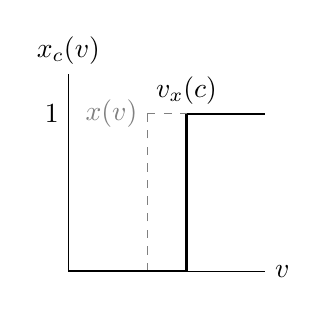
\begin{tikzpicture}
             \draw (0,0) -- (2.5,0) node[right] {$v$};
             \draw (0,0) -- (0,2.5) node[above] {$x_c(v)$};

             \draw[dashed, gray] (0,0) -- (1,0);
             \draw[dashed, gray] (1,2) -- (2.5,2);
             \draw[dashed, gray] (1,0) -- (1,2);

             \draw[thick] (0,0) -- (1.5,0);
             \draw[thick] (1.5,2) -- (2.5,2);
             \draw[thick] (1.5,0) -- (1.5,2);
             \node[above] at (1.5,2) {$v_x(c)$};

             \node[left] at (0,2) {$1$};
             \node[left, gray] at (1,2) {$x(v)$};
         \end{tikzpicture}
         \caption{
             $\mathbf{\mathbf{x_c(v)}}$: Allocates the item using single parameter allocation rule $x(v)$ if the value is at least minimal value to particpate with $v_x(c)$.
         }
     \end{subfigure}
     \caption{
         Visualization of $v_x(c)$ and the induced allocation rule $x_c(v)$.
     }
     \label{fig:visualization-of-induced-mechanism}
 \end{figure}

 If we now define a virtual value function that is conditional on $c$, by using the conditional cumulative distribution $\bar{F}_c$ and the conditional density function $\hat{f}_c$ as
 $\varphi_c(v) = v - \frac{1- \bar{F}_c(v)}{\hat{f}_c(v)}$ then we can express the expected revenue in the following theorem.

 \begin{theorem}[Expected Revenue \cite{primary}]
     \label{theorem:expected-revenue}
     Given any $\bar{F}$ with marginal cost distribution $G$, any mechanism $\mathcal{M}=(x,p)$, then the expected revenue $\Ex[t \sim \bar{F}]{p_c(v)}$ of the seller is

     \begin{align*}
         \mathbf{E}_{c \sim G}\left[\mathbf{E}_{v\sim\bar{F}_c}\left[x_c(v)\varphi_c(v)\right] - (1-\bar{F}_c(v_x(c))) \cdot \max\{-p_0,c\}\right] \eqdot
     \end{align*}
 \end{theorem}

 \begin{proof}
     We prove this using a case distinction and then draw the expectation.
     First start by fixing $c$ arbitrarily.

     Consider the case that $c > -p_0$. Note that $-p_0$ corresponds to a payment the buyer would get from the mechanism for participating.
     That means in the case that $c > -p_0$, we do not simply always participate, since our utility could be negative. Therefore, we also have $v_x(c) > 0$.
     We first consider the case that we participate, i.e. $v \geq v_x(c)$.
     In that case the buyer has to pay $p(v)$.
     \begin{align}
         \label{eq:payment-participating}
         p_c(v) = p(v) = v x(v) - \int_0^v x(t) dt + p_0
     \end{align}
     We use linearity of the integral and the definition of utility to express this in terms of the allocation function $x_c$.
     \begin{equation}
         \label{eq:utility-participating}
         \begin{aligned}
             \int_0^v x(t) dt & = \int_0^{v_c(x)} x(t) dt + \int_{v_c(x)}^v x(t) dt     \\
                              & = u^\mathcal{M}(v_c(x)) + p_0 + \int_{v_c(x)}^v x(t) dt \\
                              & = c + p_0 + \int_{v_c(x)}^v x(t) dt
         \end{aligned}
     \end{equation}
     Here the last step uses that $u^\mathcal{M}(v_c(x)) = c$ per definition of $v_c(x)$.
     Plugging \cref{eq:utility-participating} into \cref{eq:payment-participating} yields
     \begin{align}
         \label{eq:payment-participating-final}
         p_c(v) = v x_c(v) - \int_0^v x_c(t) dt - c \eqdot
     \end{align}
     Next we consider the case that the buyer does not participate, i.e. $v < v_x(c)$.
     In that case, the payment rule requests no payment, i.e. $p_c(v) = 0$, yet conveniently some part of the expression found before are also $0$.
     \begin{align*}
         p_c(v) = 0 = v x_c(v) - \int_0^v x_c(t) dt
     \end{align*}
     Thus, we can represent this entire case using an indicator function.
     \begin{align*}
         p_c(v) = 0 = v x_c(v) - \int_0^v x_c(t) dt - c \1{v \geq v_x(c)}
     \end{align*}
     Drawing the expectation around the value $v \sim \bar{F}_c$ while keeping the participation cost still fixed yields
     \begin{equation}
         \label{eq:expected-revenue-first-case}
         \begin{aligned}
             \Ex[v \sim \bar{F}_c]{p_c(v)} & = \Ex[v \sim \bar{F}_c]{v x_c(v) - \int_0^v x_c(t) dt - c \1{v \geq v_x(c)}}   \\
                                           & = \Ex[v \sim \bar{F}_c]{v x_c(v) - \int_0^v x_c(t) dt} - \Pr{v \geq v_x(c)}c   \\
                                           & = \Ex[v \sim \bar{F}_c]{x_c(v) \varphi_c(v)} - (1 - \bar{F}_c(v_x(c))) \cdot c \eqcomma
         \end{aligned}
     \end{equation}
     where in the last step we used that for fixed $c$, $\mathcal{M}_c$ is a truthful mechanism thus we can apply \cref{lemma:myerson-revenue}, simultaneously we use the definition of the cumulative distribution.

     Now we consider the opposite case, that is $c \leq -p_0$.
     Analogously to the case before, $c \leq -p_0$ means that the mechanism's payment for simply participating already pays of our participation cost.
     Certainly in that case $v_x(c) = 0$ and the buyer always participates and pays $p(v)$.
     Since $v_x(c) = 0$, we have $x_c(v) = x(v)$ for all $v \in \RR_{\geq 0}$, therefore
     \begin{align*}
         p_c(v) = p(v) = v x(v) - \int_0^v x(t)dt + p_0 = v x_c(v) - \int_0^v x_c(t)dt + p_0 \eqdot
     \end{align*}
     Drawing again the expectation around the value $v \sim \bar{F}_c$ while keeping the participation cost still fixed yields
     \begin{equation}
         \label{eq:expected-revenue-second-case}
         \begin{aligned}
             \Ex[v \sim \bar{F}_c]{p_c(v)} & = \Ex[v \sim \bar{F}_c]{v x_c(v) - \int_0^v x_c(t)dt + p_0}                  \\
                                           & = \Ex[v \sim \bar{F}_c]{x_c(v) \varphi_c(v)} + p_0                           \\
                                           & = \Ex[v \sim \bar{F}_c]{x_c(v) \varphi_c(v)} + (1 - \bar{F}_{c}(v_x(c))) p_0 \eqcomma
         \end{aligned}
     \end{equation}
     where in the last equality, we used that since $v_x(c) = 0$, $\bar{F}_{c}(v_x(c)) = 0$ as well.

     Now we can finally draw the expectation around the previously fixed $c$, combine \cref{eq:expected-revenue-first-case} and \cref{eq:expected-revenue-second-case} to get the wished theorem.
     \begin{align*}
         \Ex{p_c(v)} & = \Ex[c \sim G]{\Ex[v \sim \bar{F}_c]{x_c(v) \varphi_c(v)} + (1 - \bar{F}_{c}(v_x(c))) \max\{c, -p_0\} }
     \end{align*}
 \end{proof}

 Since we focus on revenue maximization, it is w.l.o.g. to consider $p_0 \geq 0$ \cite{primary}.
 Further \citet{primary} showed that for any mechanism with $p_0 \geq 0$ there exists a mechanism with weakly higher revenue that has $p_0 = 0$.
 Therefore, from now on, we disregard $p_0$.

 \subsection{Revenue Maximization}
 \label{sec:revenue-maximization}

 We observe that this problem is inherently non-convex.
 Even more, \citet{primary} showed that for multiple buyer it is not even representable as a convex program in general.
 Due to that, we cannot hope to calculate revenue optimal mechanisms in general in polynomial time.
 \citet{primary} propose to introduce a fully polynomial-time approximation scheme (FPTAS).

 First we focus on type distributions $\bar{F}$ where $v$ is normalized to $[0,1]$.
 Next, let $\epsilon \in (0, 1)$ be the approximation degree.
 Let $\bar{F}'$ be the value distribution with the value rounded down to the nearest multiple of $\epsilon$.
 Since there are still infinitely many allocation functions, we discretize those as well by only allocating multiples of $\epsilon$.

 This leads us to a problem definition for which an optimal mechanism is computable in polynomial time with respect to $\frac{1}{\epsilon}$.
 We will see later how to do this.
 Still it is not clear that this mechanism is close to the optimal mechanism for the original problem, here \cref{theorem:approximation-guarantee} comes into play.

 \begin{theorem}
     \label{theorem:approximation-guarantee}
     Let $\mathrm{Rev}(\bar{F}, \mathcal{M})$ be the revenue of mechanism $\mathcal{M}$ on type distribution $\bar{F}$.
     For any type distribution $\bar{F}$ supported on $[0,1]^2$, for any $\epsilon \in (0,1)$,
     the optimal mechanism $\mathcal{M}'$ on $\bar{F}'$ that only allocates multiples of $\epsilon$ and having a monotone allocation rule, achieves an expected revenue $\mathrm{Rev}(\bar{F},\mathcal{M}')$ of at least
     $\mathrm{OPT}(\bar{F}) - 4\epsilon$, where $\mathrm{OPT}(\bar{F})$ refers to the optimal expected revenue on $\bar{F}$.
 \end{theorem}

 To prove this theorem we make use of the following lemmas without proofs.

 \begin{lemma}[\citet{primary}]
     \label{lemma:allocation-function-within-e}
     For any distribution $\bar{F}$ supported on $[0,1]^2$ and for any pair of mechanisms $\mathcal{M}'$ and $\widehat{\mathcal{M}}$
     with allocation rules $x'$ and $\hat{x}$, s.t. $x'(v) \in [\hat{x}(v), \hat{x}(v) + \epsilon]$ for all $\epsilon$, we have $\mathrm{Rev}(\bar{F}, \mathcal{M}') \geq \mathrm{Rev}(\bar{F}, \widehat{\mathcal{M}}) - \epsilon$.
 \end{lemma}
 \begin{lemma}[\citet{primary}]
     \label{lemma:difference-in-optimal-mechanisms}
     Let $(\Omega, \mathcal{F}, P)$ be any probability measure and let $t_1, t_2: \Omega \rightarrow \mathbb{R}^2$ be two 2-dimensional random variables.
     If $\sup_{\omega \in \Omega} || t_1(\omega) - t_2(\omega) ||_\infty \leq \epsilon$, then $|\mathrm{OPT}(t_1) - \mathrm{OPT}(t_2)| \leq 3\epsilon$.
 \end{lemma}

 \begin{proof}[Proof of \Cref{theorem:approximation-guarantee}.]
     For any $\bar{F}$, let $\mathcal{M}'$ be the optimal mechanism on the discretized type distribution $\bar{F}'$ for which the allocation rule is also discretized.
     First, since we defined $\bar{F}'$ as the \textit{rounded down} type distribution, for any mechanism $\mathcal{M}$ with monotone allocation rule holds, that $\mathrm{Rev}(\bar{F}, \mathcal{M}) \geq \mathrm{Rev}(\bar{F}', \mathcal{M})$, so in particular this also applies to $\mathcal{M}'$.

     Next, we define $\widehat{\mathcal{M}}$ as the optimal mechanism on $\bar{F}'$ (one that is allowed to allocate continuous values).
     We use \cref{lemma:allocation-function-within-e}, since our allocation function $x'$ of mechanism $\mathcal{M}'$
     allocates within an $\epsilon$-interval of the allocation function $\hat{x}$ of $\widehat{\mathcal{M}}$.
     Thus, according to \cref{lemma:allocation-function-within-e}, we got $\mathrm{Rev}(\bar{F}', \mathcal{M}') \geq \mathrm{Rev}(\bar{F}', \widehat{\mathcal{M}}) - \epsilon$.

     Finally, note, that for the two type distributions $\bar{F}$ and $\bar{F}'$ it holds that they originate from the same probability measure, yet the value of the random variables differs by at most $\epsilon$.
     Also note, that we did not round the participation cost, thus the difference with respect to the infinity-norm $|| \cdot ||_{\infty}$ is also at most $\epsilon$.
     Therefore, we can apply \cref{lemma:difference-in-optimal-mechanisms}, since $\widehat{\mathcal{M}}$ is optimal mechanism on $\bar{F}'$,
     to get $\mathrm{Rev}(\bar{F}', \widehat{\mathcal{M}}) \geq \mathrm{OPT}(\bar{F}') - 3\epsilon$.

     Putting everything together yields the stated approximation guarantee
     \begin{align*}
         \mathrm{Rev}(\bar{F}, \mathcal{M}') & \geq \mathrm{Rev}(\bar{F}', \mathcal{M}')                     \\
                                             & \geq \mathrm{Rev}(\bar{F}', \widehat{\mathcal{M}}) - \epsilon \\
                                             & \geq \mathrm{OPT}(\bar{F}') - 4\epsilon \eqdot
     \end{align*}
 \end{proof}

 Now that we know that the difference in the problem statement leads to a reasonable approximation guarantee,
 we can dedicate ourselves to finding an optimal mechanism for this problem.

 We will use a dynamic program based on the approximation degree $\epsilon$ to calculate for all possible valuations
 an allocation function that optimizes the revenue.
 We will make sure this allocation rule is non-decreasing and will follow the payment rule through \cref{lemma:thruthful-mechanism}
 in order to also get a truthful mechanism.
 Note that \cref{lemma:thruthful-mechanism} also tells us, that it is enough to find a single parameter allocation rule and optimize the revenue of the induced mechanism $\mathcal{M}_c$ with payment rule $p_c$.

 For integers $i,j \leq \frac{1}{\epsilon}$ and $k \leq \frac{1}{\epsilon^2}$,
 we define $R(i,j,k)$ as the optimal revenue from only a subset of the buyers, those that have a value $v \leq i \epsilon$
 and while the allocation function is fixed for $i\epsilon$ to $x(i \epsilon) = j \epsilon$ and the utility is also fixed to $u(i \epsilon) = k \epsilon^2$.
 Observe that this informal definition is equivalent to
 \begin{equation}
     \label{eq:rijk}
     R(i,j,k) = \max_{\mathcal{M}: x(i\epsilon) = j\epsilon, u(i\epsilon) = k \epsilon^2} \Pr{v \leq i\epsilon}\Ex{p_c(v)\mid v \leq i \epsilon} \eqdot
 \end{equation}

 \begin{theorem}
     \label{theorem:recursion-formular}
     For $i \geq 2$, $R(i,j,k)$ can be calculated as
     \begin{align*}
         R(i,j,k) = \max_{j' \leq j} R(i-1, j, k - j) + q_i \bar{F}_i'(k \epsilon^2) \cdot (i\cdot j - k)\epsilon^2 \eqcomma
     \end{align*}
     where $q_i$ refers to the occurrence probability of $v = i \epsilon$ and $\bar{F}_i'$ refers to the cumulative type distribution conditional on the value being $i\epsilon$.
 \end{theorem}

 See \cref{fig:fptas-recursion-formular} for a visualization of this theorem.

 \begin{figure}[htp!]
     \centering
     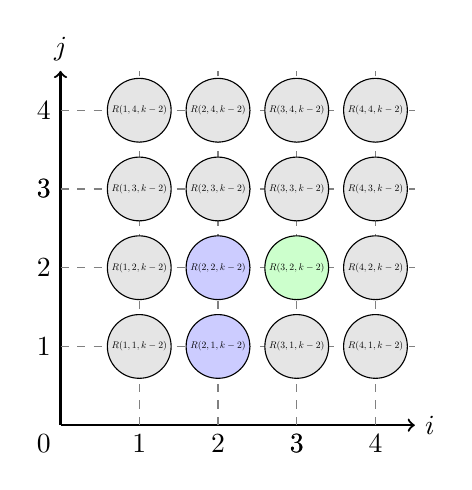
\begin{tikzpicture}[
             node/.style={circle, draw=black, fill=gray!20, scale=.35},
             axis/.style={->, thick},
             gridline/.style={gray, dashed}
         ]

         \draw[axis] (0, 0) -- (4.5, 0) node[right] {$i$};
         \draw[axis] (0, 0) -- (0, 4.5) node[above] {$j$};

         \foreach \x in {1, 2, 3, 4} {
                 \draw[gridline] (\x, 0) -- (\x, 4.5);
                 \draw[gridline] (0, \x) -- (4.5, \x);
             }

         \foreach \i in {1, 2, 3, 4} {
                 \foreach \j in {1, 2, 3, 4} {
                         \ifthenelse{\i=3\and\j=2}
                         {
                             \node[node, fill=green!20] at (\i, \j) {$R(\i,\j,k -2)$};
                         }
                         {
                             \ifthenelse{\i=2\and\j<3}
                             {
                                 \node[node, fill=blue!20] at (\i, \j) {$R(\i,\j,k - 2)$};
                             }
                             {
                                 \node[node] at (\i, \j) {$R(\i,\j,k - 2)$};
                             }
                         }
                     }
             }

         \node at (0, 0) [below left] {0};
         \foreach \x in {1, 2, 3, 3, 4} {
                 \node at (0, \x) [left] {\x};
                 \node at (\x, 0) [below] {\x};
             }
     \end{tikzpicture}
     \caption{
         Visualization of \Cref{theorem:recursion-formular}. For $R(3,2,k)$ we need to maximize over all $R(2, j', k-j)$ where $j' \leq j = 2$.
     }
     \label{fig:fptas-recursion-formular}
 \end{figure}

 From this we can directly deduce the following corollary.

 \begin{corollary}
     The optimal mechanism $\mathcal{M}'$ that only allocates multiples of $\epsilon$ on any discretized type distribution $\bar{F}'$
     can be computed in $\mathcal{O}\left(\frac{1}{\epsilon^5}\right)$.
 \end{corollary}
 \begin{proof}
     Observe that from the definition of $R(i,j,k)$, it holds that
     \begin{align*}
         \mathrm{Rev}(\bar{F}', \mathcal{M}') = \max_{j \leq \frac{1}{\epsilon}, k \leq \frac{1}{\epsilon^2}} R\left(\frac{1}{\epsilon}, j, k\right) \eqdot
     \end{align*}

     Using dynamic programming by applying \cref{theorem:recursion-formular} and fixing the base cases $R(1,j,k) = 0$ for any $k \leq j$ and $R(1,j,k)=-\infty$ for any $k > j$,
     we can calculate for all $\frac{1}{\epsilon^4}$ combinations of $i,j$ and $k$ the respective values of $R(i,j,k)$.
     Each of those $R(i,j,k)$ needs at most $\frac{1}{\epsilon}$ calculations because of the maximum.
     Therefore, we calculate the revenue of $\mathcal{M}'$ in $\mathcal{O}\left(\frac{1}{\epsilon^5}\right)$ time.
     Recovering the actual mechanism $\mathcal{M}'$ and its allocation rule from that is simply a matter of backtracking the $j'$ that maximized our expression.
 \end{proof}

 All that is left is to prove \cref{theorem:recursion-formular}.
 \begin{proof}[Proof of \Cref{theorem:recursion-formular}]
     First recall the definition of $R(i,j,k)$.
     \begin{align*}
         R(i,j,k) = \max_{\mathcal{M}: x(i\epsilon) = j\epsilon, u(i\epsilon) = k \epsilon^2} \Pr{v \leq i\epsilon}\Ex{p_c(v)\mid v \leq i \epsilon}
     \end{align*}
     Observe that we can use the linearity of expectation to split up the expectation of \cref{eq:rijk} into the case that $v \leq (i-1)\epsilon$ and the case that $v = i \epsilon$.
     \begin{align*}
          & \Ex{p_c(v)\mid v \leq i \epsilon}                                                           \\
          & = \Pr{v \leq (i-1)\epsilon \mid v \leq i \epsilon} \Ex{p_c(v) \mid v \leq (i - 1) \epsilon} \\
          & + \Pr{v = i \epsilon \mid v \leq i \epsilon} \Ex{p_c(v) \mid v = i \epsilon}
     \end{align*}
     Next if we pull in the $\Pr{v \leq i\epsilon}$ it neatly cancels out the condition on the probabilities, leading to
     \begin{align*}
           & R(i,j,k)                                                                                                                                                                                             \\
         = & \max_{\mathcal{M}: x(i\epsilon) = j\epsilon, u(i\epsilon) = k \epsilon^2} (\Pr{v \leq (i-1)\epsilon} \Ex{p_c(v) \mid v \leq (i - 1) \epsilon} + \Pr{v = i \epsilon} \Ex{p_c(v) \mid v = i \epsilon}) \eqdot
     \end{align*}
     Further, observe that for $p_c(v)$ in the second expectation, everything is already fixed with the maximization constraints, i.e. for the fixed value $v = i \epsilon$ the allocation is fixed and the utility is fixed, thus also the payment.
     This means, we can pull out the second term, since the maximization does not affect it.
     So, we can focus on the term $\max_{\mathcal{M}: x(i\epsilon) = j\epsilon, u(i\epsilon)=k\epsilon^2} \Pr{v \leq (i-1)\epsilon} \Ex{p_c(v) \mid v \leq (i - 1) \epsilon}$ on its own.

     Note that this is similar to \cref{eq:rijk} with $v = (i-1) \epsilon$, only the maximization constraints differ.
     For that we only need to fix $x((i-1)\epsilon)$ and $u((i-1)\epsilon)$.
     Conveniently, we can express the latter in terms of things that are already fixed.
     Note that we can write $u(i\epsilon)$ as
     \begin{align*}
         u(i\epsilon) & = \int_0^{i\epsilon} x(t) dt                                             \\
                      & = \int_0^{(i-1)\epsilon} x(t) dt + \int_{i-1\epsilon}^{i\epsilon} x(t)dt \\
                      & = u((i-1)\epsilon) + \epsilon j \epsilon^2 \eqcomma
     \end{align*}
     where in the last the step we used that $x(i\epsilon) = j\epsilon$.
     Rearranging this, yields
     \begin{align*}
         u((i-1)\epsilon) = u(i\epsilon) - j \epsilon^2 = (k - j) \epsilon^2 \eqdot
     \end{align*}
     For $x((i - 1)\epsilon)$ one cannot find a direct solution derived from the constraints of $x(i\epsilon)$, thus we apply an actual maximization here.
     However, we must ensure that $x$ is non-decreasing, thus $j' \epsilon = x((i-1)\epsilon) \leq x(i\epsilon) = j\epsilon$.

     Combining this yields for the first term
     \begin{align*}
         \max_{\mathcal{M}: x(i\epsilon) = j\epsilon, u(i\epsilon) = k \epsilon^2} \Pr{v \leq (i-1)\epsilon} \Ex{p_c(v) \mid v \leq (i - 1) \epsilon} = \max_{j' \leq j} R(i-1, j, k - j) \eqdot
     \end{align*}

     Next we focus on the second term $\Pr{v = i \epsilon} \Ex{p_c(v) \mid v = i \epsilon}$ given that $x(i\epsilon) = j\epsilon$ and $u(i\epsilon) = k\epsilon^2$.
     $\Pr{v = i \epsilon} = q_i$ per definition of $q_i$.
     The expected revenue given that $v = i \epsilon$ depends on the event that the buyer participates.
     She only does this, if her participation cost is higher than the utility gain from the single-parameter mechanism.
     In other words
     \begin{align*}
          & \Ex{p_c(v) \mid v = i \epsilon}_{x(i\epsilon) = j \epsilon, u(i\epsilon) = k\epsilon^2}                                         \\
          & = \Pr{c \geq u(i\epsilon)} \Ex{p_c(i\epsilon) \mid c \leq u(i\epsilon)}_{x(i\epsilon) = j \epsilon, u(i\epsilon) = k\epsilon^2} \\
          & = \bar{F}_i'(k\epsilon^2) \Ex{p(i\epsilon)}_{x(i\epsilon) = j \epsilon, u(i\epsilon) = k\epsilon^2}                             \\
          & = \bar{F}_i'(k\epsilon^2) \Ex{u(i\epsilon) - i\epsilon \cdot x(i\epsilon)}                                                      \\
          & = \bar{F}_i'(k\epsilon^2) (k - i \cdot j)\epsilon^2 \eqdot
     \end{align*}
     This simplifies the second term to
     \begin{align*}
           & \Pr{v = i \epsilon} \Ex{p_c(v) \mid v = i \epsilon}_{x(i\epsilon) = j \epsilon, u(i\epsilon) = k\epsilon^2} \\
         = & q_i \bar{F}_i'(k\epsilon^2) (k - i \cdot j)\epsilon^2 \eqdot
     \end{align*}
     Combining both terms proves our theorem.
     \begin{align*}
         R(i,j,k) = \max_{j' \leq j} R(i-1, j, k - j) + q_i \bar{F}_i'(k \epsilon^2) \cdot (i\cdot j - k)\epsilon^2
     \end{align*}
 \end{proof}

 \subsection{Reduction to Multiple Buyer}
 Using the mechanism designed in \cref{sec:revenue-maximization} for a single buyer, \citet{primary} derive an approximate algorithm for multiple buyers.
 For that they use that any algorithm allocating a single item to multiple buyers allocates the item in expectation to at most once.
 Therefore, the sum of ex-ante probabilities for allocating it to each buyer is also at most $1$.
 One now splits the probabilities into shares for each buyer while maximizing the revenue.
 After that each buyer is approached sequentially with the single parameter mechanism from \cref{sec:revenue-maximization}.
 The mechanism is modified, s.t. the item is only allocated with the precomputed probability to each buyer.
 This general reduction scheme was first proposed by \citet{alaei2012bayesian,alaei2014bayesian} leads to a $\frac{1}{2}\mathrm{OPT} - \epsilon$ approximation of the optimal mechanism in $\mathrm{poly}\left(\frac{1}{\epsilon}\right)$ computation time in our case.
\end{section}

\begin{section}{Conclusion}
 This article introduced the model of private participation costs to single item auctions.
 In particular the focus lied on single item, single buyer auctions.
 First we characterized how regular single parameter truthful mechanisms can be employed on the model of private participation costs.
 Based on that, we derived the expected revenue for seller employing such mechanisms, yet noticed that the problem is non-convex.
 Due to that we approached the revenue maximization problem in an approximate manner, by discovering a FPTAS \cite{primary}.
 This FPTAS uses a dynamic program to compute a $\mathrm{OPT}-4\epsilon$ approximation of the optimal revenue in $\mathcal{O}\left(\frac{1}{\epsilon^5}\right)$ time.
 Finally, we motivated how \citet{primary} used a sequential-opt-out-mechanism to solve the multiple buyers' problem approximately using the single buyer's FPTAS.
\end{section}

\bibliography{references} % Insert name of .bib file

\end{document}
